Malta se ha convertido en uno de los mayores lugares turísticos de Europa, y, por tanto, el explorar nuevas tecnologías que ayuden a quienes lo aprenden se vuelvan proficientes en el maltés en lo más rápido posible, es un área relevante de investigación. El aprendizaje de lenguajes con la RV no solo se limita a los estándares tradicionales de la educación, esta puede crear experiencias de aprendizaje inmercidas e interactivas fuera del salón de clases, como lo pueden ser experiencias culturales. La RV facilita el aprendizaje de lenguajes en contextos específicos, como lo puede ser ajustado hacia negocios o profesionalmente. La RV debería de utilizarse como una herramienta complementaria, ya que, potencialmente, se puede caer en adicciones a este tipo de dispositivos, y no debería de reemplazar completamente a un profesor. \cite{ZAMMIT2023100035}

\begin{figure}[H]
   \begin{center}
      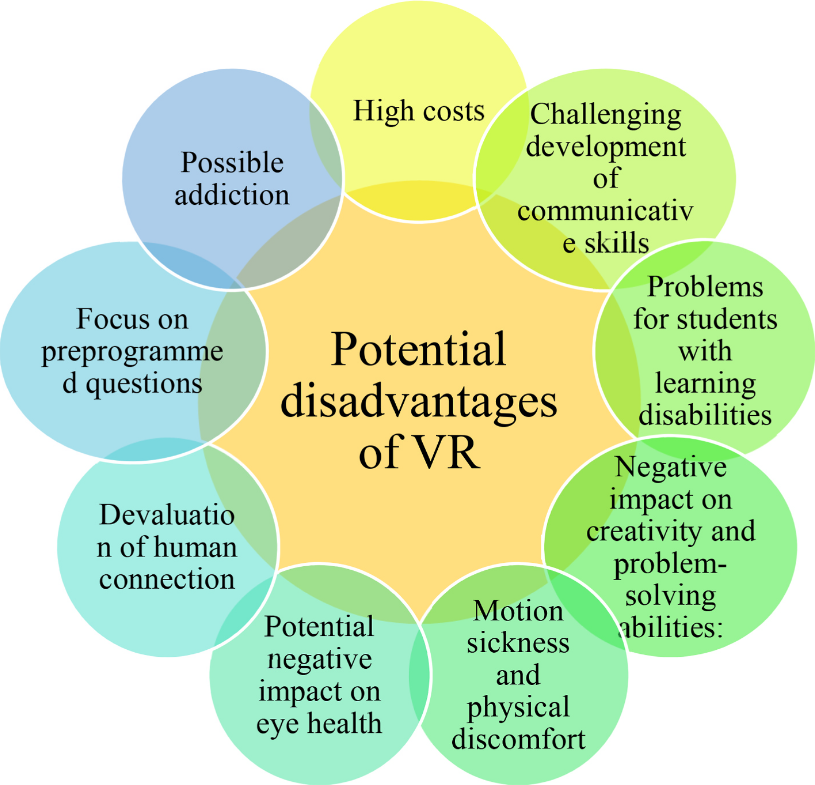
\includegraphics[scale=0.2]{Archivos/exploring-the-effectiveness-of-virtual-reality-in-teaching-maltese-fig-2.png}
   \end{center}
   \caption{Las desventajas de la RV}
   \label{fig:disvr}
   \textit{Nota. }Imagen extraída de \cite{ZAMMIT2023100035}
\end{figure}

